\documentclass[12pt,a4paper]{report}
%
% This LaTeX template has been created by Luca Grilli
% Based on the following https://en.wikibooks.org/wiki/LaTeX/Title_Creation
%
\usepackage[italian]{babel}
%\usepackage[T1]{fontenc} % Riga da commentare se si compila con PDFLaTeX
\usepackage[
top    = 4.00cm,
bottom = 2.00cm,
left   = 3.00cm,
right  = 3.00cm]{geometry}
%\usepackage{geometry}
\usepackage{graphicx}
\usepackage{hyperref}
\usepackage[utf8]{inputenc}
\usepackage{subcaption}
\usepackage[nottoc,numbib]{tocbibind}
\usepackage{titlesec}
\usepackage{algorithm}
\usepackage{algpseudocode}
\usepackage{float}


\titleformat{\chapter}[display]{\Huge\bfseries}{}{0pt}{\thechapter.\ }
\titlespacing{\chapter}{0pt}{-32pt}{1cm}



\graphicspath{{figures/}}
%
%\addtolength{\topmargin}{-.875in} % reduce the default top margin
\addtolength{\topmargin}{-2cm} % reduce the default top margin
%



%%%%%%%%%%%%%%%%%%%%%%%%%%%%%%%%%%
%                                %
%     Begin Document [start]     %
%                                %
%%%%%%%%%%%%%%%%%%%%%%%%%%%%%%%%%%
\begin{document}


%%%%%%%%%%%%%%%%%%%%%%%%%%%%%%
%     Title Page [start]     %
%%%%%%%%%%%%%%%%%%%%%%%%%%%%%%
% Declare new geometry for the title page only.
%\newgeometry{margin=1in}
\begin{titlepage}
	\centering
	\includegraphics[width=0.30\textwidth]{logo-unipg}\par\vspace{0.5cm}
	\large{Tesina Finale di}\par
	\large{\textbf{Algoritmi e Strutture Dati}}\par
	\small{Corso di Laurea in Ingegneria Informatica ed Elettronica -- A.A. 2023-2024}\par
	\textsc{\small{Dipartimento di Ingegneria}}\par 
	%\large{A.A. 2018-2019}\par

	%\vfill
	\vspace{0.5cm}
	docente\par
	Prof.~Emilio \textsc{Di Giacomo}

	\vspace{1cm}
	\vspace{1cm}
	\textbf{\huge{A* Pathfinding}}\par
	\vspace{0.2cm}
	Implementazione di algoritmi per la generazione di grafi e ricerca del cammino minimo\par
	\vspace{0.5cm}
	%\includegraphics[width=0.30\textwidth]{TODOlogo}\par\vspace{1cm}
	\vspace{1cm}

	\large{Studente}\par
	\vspace{0.5cm}
	\large{311462}
	\large{\textbf{Andrea Zonghi}}
	\large{andrea.zonghi@studenti.unipg.it}\\

	\vfill
	%Bottom of the page
	%{\large \today\par}
	\raggedright
	\small{Data ultimo aggiornamento: \today}
\end{titlepage}
% Ends the declared geometry for the titlepage
\restoregeometry
%%%%%%%%%%%%%%%%%%%%%%%%%%%%
%     Title Page [end]     %
%%%%%%%%%%%%%%%%%%%%%%%%%%%%

%%%%%%%%%%%%%%%%%%%%%%%%%%
%     Indice [start]     %
%%%%%%%%%%%%%%%%%%%%%%%%%%
\tableofcontents
%%%%%%%%%%%%%%%%%%%%%%%%
%     Indice [end]     %
%%%%%%%%%%%%%%%%%%%%%%%%

%%%%%%%%%%%%%%%%%%%%%%%%%%%%%%%%%%%%%%%%%%%%
%     Descrizione del Problema [start]     %
%%%%%%%%%%%%%%%%%%%%%%%%%%%%%%%%%%%%%%%%%%%%
\chapter{Descrizione del problema}\label{ch:des-pro}
Nella teoria dei grafi la ricerca del cammino minimo tra due vertici di un grafo \(G = (V, E)\) consiste nel trovare un percorso che va dal primo al secondo tale che la somma dei pesi degli archi che lo costituiscono sia minima.
La proprietà su cui si fondano gli algoritmi per il calcolo dei cammini minimi è che il sottocammino di un cammino minimo è anch'esso un cammino minimo.
Inoltre alcuni algoritmi restringono i pesi ad essere solamente positivi, oppure accettano archi con peso anche negativo ma poi segnalano la presenza di cicli negativi che impediscono di calcolare la soluzione corretta.

Abbiamo diverse varianti di questo problema, tra cui cercare: il cammino minimo tra un vertice e tutti gli altri appartenenti al grafo (sorgente unica), tra ciascun vertice ed una singola destinazione (destinazione unica, uguale al precedente invertendo la direzione degli archi), tra una coppia di vertici e tra tutte le coppie di vertici.

Il problema su cui ci concentreremo in questa tesina è quello del cammino minimo tra due vertici in grafi con diverse caratteristiche (sparsi, densi, orientati e non orientati).

%----------------------------------------
% Sezione: Algoritmi di Pathfinding Analizzati [start]
%----------------------------------------
\section{Algoritmi di Pathfinding Analizzati}\label{se:algo-path-anal}
Esistono molti algoritmi di pathfinding tra due nodi con pesi non uniformi ed hanno tutti caratteristiche e realizzazioni differenti. 
Tra i più noti troviamo l'algoritmo di Dijkstra che si concentra sulla risoluzione del problema della sorgente unica, non accettando pesi degli archi negativi. 
Nella versione che utilizza heap di Fibonacci è al momento l'algoritmo più veloce (asintoticamente) conosciuto per questa computazione, considerando grafi diretti arbitrari e pesi potenzialmente illimitati, avendo una complessità temporale pari a $\Theta (|E|+|V|\log |V|)$. 
Per casi più particolari ci sono specializzazioni adatte dell'algoritmo che lo rendono più efficiente in quelle specifiche condizioni. 
L'idea generale del funzionamento dell'algoritmo è quella di partire dal nodo sorgente ed assegnare a questo un peso 0, mentre a tutti gli altri nodi si assegna una distanza inizialmente infinita. 
Poi ad ogni passaggio si seleziona il nodo con il peso minore dall'insieme dei nodi non ancora visitati e si aggiornano le distanze di tutti i nodi adiacenti a questo, applicando anche la tecnica del rilassamento \cite{baeldungEdgeRelaxation}, e si tiene traccia del percorso per raggiungere questi nodi. 
In seguito si marca il nodo scelto come visitato e si rimuove dall'insieme dei nodi non visitati. 
Si ripetono quindi questi passaggi finché tutti i nodi vengono visitati. 
Infine si possono ricostruire le distanze dai nodi alla sorgente utilizzando i dati raccolti durante l'aggiornamento della distanza.

\medskip

Un altro algoritmo in parte simile per risolvere lo stesso problema è quello di Bellman e Ford. 
Questo è più versatile di Dijkstra sotto un certo punto di vista, in quanto accetta che alcuni archi abbiano peso negativo. 
La presenza di cicli negativi raggiungibili dalla sorgente fa però sì che non esistano cammini minimi in quanto basterebbe attraversare ripetutamente il ciclo per diminuire il costo totale. 
In questo caso Bellman-Ford rileva il ciclo negativo e lo segnala. 
Il funzionamento è diverso da Dijkstra in quanto si effettua il rilassamento di ogni arco del grafo per \(V-1\) volte, dove V è il numero di nodi del grafo. 
Dopo questo processo si fa un ulteriore rilassamento di tutti gli archi e se si trova ancora un miglioramento nelle distanze questo significa che ci sono cicli di peso negativo raggiungibili dal nodo sorgente.
Per quanto riguarda l'efficienza questo è sicuramente meno efficiente del precedente in quanto richiede, nel caso peggiore, $\Theta (|V||E|)$ operazioni, dove V è il numero dei nodi ed E è il numero degli archi.

Entrambi questi due algoritmi precedentemente analizzati si possono adattare per cercare il percorso minimo tra un nodo sorgente ed una destinazione, basta usare come condizione di terminazione l'aver o meno determinato la distanza minima del nodo di destinazione. 

\medskip

Il prossimo algoritmo invece è specifico per il problema del pathfinding tra tutte le coppie di vertici ed è l'algoritmo di Floyd e Warshall, che accetta anche archi con peso negativo (non cicli negativi però). 
Per quanto riguarda il funzionamento si costruisce una matrice delle distanze di dimensione VxV e si inizializzano tutte le distanze da un nodo a sé stesso uguali a zero.
La distanza tra due nodi collegati da un arco è rappresentata come l'elemento [i][j] della matrice ed è impostata al peso conosciuto di quell'arco. 
Nel caso in cui non ci sia un arco tra due nodi, la distanza è inizialmente impostata ad infinito. 
L'algoritmo quindi esegue un numero V di iterazioni ed in ciascuna iterazione k considera tutti i nodi \textit{i} e \textit{j}. 
Per ogni coppia \textit{(i,j)} si controlla se passando per il nodo k si ha un percorso più breve rispetto a quello già conosciuto e in caso si aggiorna.
Al termine delle V operazioni quindi la matrice delle distanze contiene la distanza minima tra tutte le coppie dei nodi.
Per quanto riguarda la complessità abbiamo un tempo \textbf{\textit{$O(V^3)$}} ed un'occupazione di spazio pari a \textbf{\textit{$O(V^2)$}}.

Anche quest'ultimo algoritmo si può usare per calcolare il percorso minimo tra due vertici, ma sarebbe particolarmente inefficiente in quanto abbiamo una sola coppia nodi.

\medskip

Arriviamo quindi infine all'algoritmo A* che risolve specificatamente il problema di pathfinding che stiamo analizzando.
Questo combina l'algoritmo di Dijkstra con la ricerca best-first, utilizzando una funzione euristica per la stima della distanza del nodo dalla destinazione. 
Questa in pratica aiuta l'algoritmo a muoversi efficientemente verso la destinazione.
La scelta dell'euristica è fondamentale e questa deve essere ammissibile, cioè non deve mai sovrastimare il reale costo per garantire che il percorso stimato sia ottimo.
Il funzionamento è praticamente lo stesso di Dijkstra, ma per ogni nodo \textit{n} si calcola il costo stimato \textit{f(n)} come somma del costo esatto del percorso dal nodo iniziale al nodo n più la stima euristica del costo dal nodo n alla destinazione.
Si prende quindi dall'insieme dei nodi da visitare quello con il costo stimato \textit{f(n)} minore e si esplora, aggiornando i nodi ad esso adiacenti.
Per ogni nodo vicino \textit{m} si calcola un nuovo valore \textit{g(m)} come somma del costo esatto del percorso del nodo iniziale al nodo n più il costo dell'arco che collega n ad m. 
Se questo nuovo valore è inferiore a quello precedentemente noto per m, si aggiorna g(m) e si calcola f(m), impostando anche n come predecessore di m per poter ricostruire il percorso.
Infine si aggiunge (o aggiorna) m nell'insieme dei nodi da visitare.
L'algoritmo termina quando il nodo di destinazione è quello con il costo stimato f(n) minore e viene scelto come prossimo nodo da esplorare oppure quando non ci sono più percorsi da visitare.
La complessità temporale dipende fortemente dalla qualità dell'euristica utilizzata e, con una buona funzione, può essere significativamente più veloce di Dijkstra. Se il grafo è un albero e con una funzione f che rispetta la condizione \textbf{\textit{$|f(x)-f^{*}(x)|=O(\log f^{*}(x))$}}, dove \textit{f*} è l'euristica ottimale cioè l'esatta distanza per andare da x all'obiettivo, la complessità temporale è \textbf{polinomiale}.
Un problema potrebbe però essere la complessità spaziale \textbf{\textit{$O(|V|)$}}, in quanto nel caso peggiore può essere necessario tenere tutti i nodi in memoria.

Utilizzeremo quindi questo ultimo algoritmo, A*, per il problema della ricerca del cammino minimo tra due nodi che stiamo studiando.
%----------------------------------------
% Sezione: Algoritmi di Pathfinding Analizzati [end]
%----------------------------------------

%------------------------------------------------------------%
% Sezione: Algoritmi di Generazione Grafi Analizzati [start] %
%------------------------------------------------------------%
\section{Algoritmi di Generazione Grafi Analizzati}\label{se:algo-gen-anal}
Un primo approccio alla generazione di grafi potrebbe essere quello di, dato un numero $N^2$ di nodi, generare un grafo a griglia creando una matrice NxN dove ogni cella $(i,j)$ rappresenta un singolo vertice di coordinate i e j. 
Inoltre possiamo aggiungere le celle (i-1,j), (i,j+1), (i+1,j) e (i,j+1) in una lista o matrice di adiacenza per rappresentare gli archi ai quattro nodi vicini.
In questo caso potremmo anche decidere arbitrariamente di rimuovere degli archi per ridurre la densità del grafo e bloccare alcuni passaggi.

Sarebbe sicuramente un metodo efficace, ma volendo utilizzare un tipo di grafo più generico analizziamo il modello di Erdős e Rényi \cite{wikipediaErdosRenyiModel} \cite{ErdosRenyiRandomGraphs} (modello ER) per la generazione casuale di grafi.
Ci sono due varianti del modello ER che sono per alcuni tratti simili:
\begin{itemize}
    \item il modello $G(n,m)$ dove un grafo è scelto randomicamente dalla collezione contenente tutti i grafi che hanno \textbf{n} nodi e \textbf{m} archi e permutazioni diverse dei vertici sono considerate grafi diversi. Definito \textbf{T} il numero di grafi nella collezione, ogni grafo ha la stessa probabilità $P=1/T$ di essere scelto.
    \item il modello $G(n,p)$ dove un grafo è costruito connettendo due nodi a caso. Ogni arco viene incluso nel grafo con probabilità indipendente \textbf{p}. Questo parametro di probabilità \textbf{p} può essere visto come una funzione di ponderazione in quanto, aumentando p da 0 ad 1, il modello includerà con probabilità crescente grafi con più archi e con probabilità sempre più bassa grafi con meno archi.
\end{itemize}

Una importante proprietà di quest'ultimo modello è che se \(p<(1-\epsilon)ln(n)/n\) allora un grafo $G(n,p)$ conterrà quasi sicuramente vertici isolati e quindi non sarà connesso mentre se \(p>(1-\epsilon)ln(n)/n\) allora un grafo $G(n,p)$ sarà quasi sicuramente connesso. In entrambi i casi più è grande il numero di nodi n e più sarà preciso il risultato. 

Vediamo quindi che $ln(n)/n$ è un punto critico per per la connettività di $G(n,p)$.

Utilizzeremo quindi questo secondo modello ER per quando sarà necessario generare grafi.
%----------------------------------------------------------%
% Sezione: Algoritmi di Generazione Grafi Analizzati [end] %
%----------------------------------------------------------%

%%%%%%%%%%%%%%%%%%%%%%%%%%%%%%%%%%%%%%%%%%
%     Descrizione del Problema [end]     %
%%%%%%%%%%%%%%%%%%%%%%%%%%%%%%%%%%%%%%%%%%

%%%%%%%%%%%%%%%%%%%%%%%%%%%%%%%%%%%%%%%%%%%%%%%%%%%%%%%%%%%
%     Algoritmi e Strutture Dati Implementati [start]     %
%%%%%%%%%%%%%%%%%%%%%%%%%%%%%%%%%%%%%%%%%%%%%%%%%%%%%%%%%%%
\chapter{Algoritmi e Strutture Dati Implementati}\label{ch:algo-struc-impl}

Abbiamo quindi l'implementazione di due diversi algoritmi, uno per trovare il cammino minimo tra due nodi, e l'altro per la generazione di grafi a partire dal numero di vertici \textbf{n} e da una probabilità \textbf{p}. 
Viene inoltre implementato un metodo per creare un grafo a partire da due file di testo contenenti nodi ed archi in una specifica formattazione. Questo verrà poi usato per eseguire set di esperimenti con A*. Tale funzione sarà utile in quanto viene implementata anche l'opzione di creare un singolo grafo con il modello ER e salvarlo in due file di testo nella formattazione usata dal metodo precedente.

Il grafo che viene generato, letto o su cui si lavora è rappresentato da un array di nodi, implementati nel progetto nella classe \textit{Node}. Gli archi invece sono modellati dalla classe \textit{Edges}. 

In \textit{Nodes} troviamo gli attributi di base del nodo che sono: un identificativo, la coordinata X, la coordinata Y ed una lista di archi. Quest'ultima è la lista di adiacenza che serve a rappresentare il grafo ed è stata scelta al posto della matrice di adiacenza perché nell'implementazione poi successiva di A* si avrà necessità di scorrere tutti i nodi adiacenti ad uno dato, operazione in cui è più veloce della sua controparte.

Viene scelto di utilizzare una lista di archi invece della più canonica lista di adiacenza fatta di nodi perché in questa implementazione abbiamo i pesi solamente sugli archi. Questo potrebbe essere utile nel caso in cui, per esempio, dovremmo utilizzare l'algoritmo su grafi che rappresentano strade e ci permetterebbe di cambiare il peso di uno specifico tratto di strada in base alle variabili del caso (eg: condizioni di viabilità, limiti di velocità bassi) in modo piuttosto semplice.
La lista di nodi viene implementata usando un oggetto della classe \textit{ArrayList} di Java \cite{oracleArrayListJava}.

Per quanto riguarda la classe \textit{Edge} abbiamo i nodi di inizio, di fine ed il costo.

Viene poi implementata una classe \textit{Result}, utilizzata poi per ritornare i risultati dell'esecuzione di A*. In essa troviamo il percorso minimo cercato, modellato come lista di nodi, ed il suo costo complessivo.

%--------------------------------------------------------------%
% Sezione: Algoritmo A*, coda di priorità e mappa hash [start] %
%--------------------------------------------------------------%
\section{Algoritmo A*, coda di priorità e mappa hash}\label{se:a-star-coda-mappa}

Passando ad A* abbiamo innanzitutto una classe ausiliaria, chiamata \textit{NodeComp}, che implementa l'interfaccia di Java \textit{Comparable} \cite{oracleComparableJava}, necessaria per ordinare gli elementi nella coda di priorità usata dall'algoritmo. Qui troviamo un nodo, il suo predecessore, il costo dal nodo di partenza calcolato fino a quel momento ed il costo dal nodo di partenza stimato dall'euristica utilizzata.
Altro punto degno di nota in questa classe è l'override del metodo \textit{compareTo()}, necessario a far funzionare correttamente l'ordinamento della coda di priorità.
Un altro metodo ausiliario utilizzato nel codice che esegue A* è il metodo statico \textit{euclideanDistance()} che rappresenta la nostra euristica e calcola la distanza euclidea \cite{wikipediaDistanzaEuclidea} tra due punti in uno spazio bidimensionale. Per altre necessità si potrebbero usare altre euristiche, come ad esempio la distanza di Manhattan \cite{wikipediaGeometriaTaxi} se si utilizzasse il grafo a griglia visto nella \hyperref[se:algo-gen-anal]{sezione 1.2}.

Arriviamo quindi ad implementare l'algoritmo A*, che come visto prima, è praticamente una versione dell'algoritmo di Dijkstra ottimizzato per la ricerca verso un solo punto e che utilizza una funzione euristica per dirigersi nella giusta direzione. 
Come openSet viene scelta una coda di (min-)priorità, implementata con la classe \textit{PriorityQueue} di Java in quanto gli elementi al suo interno vengono ordinati secondo il costo stimato, attributo usato come termine di paragone nell'override del metodo \textit{compareTo()}.
L'openSet invece viene realizzato utilizzando la classe \textit{HashMap} di Java in quanto le operazioni \textit{get()} e \textit{put()} sono realizzate in tempi costanti con questa struttura dati. La \textit{get()} viene utilizzata sotto forma di \textit{containsKey()} per vedere se di un sono già stati presi in considerazione tutti i nodi ad esso adiacenti, mentre la \textit{put()} viene utilizzata per aggiungere elementi alla mappa.
Vediamo in dettaglio lo pseudocodice nella pagina successiva.

\newpage

\begin{algorithm}
\caption{Trova Percorso con A*}
\label{alg:A-Star}
\begin{algorithmic}[1]
    \State \textbf{Input} Nodo iniziale $start$, nodo finale $goal$
    \State \textbf{Output} Percorso più breve $path$, costo totale $totalPathCost$
    \State inizializzo una PriorityQueue vuota
    \State inizializzo una HashMap vuota
    \State $startNode=$ nuovo $NodeComp$ con costo accumulato=0 e costo stimato
    \State aggiungo startNode all'openSet
    \While{openSet non è vuoto}
        \State $next=$ nodo in cima all'openSet
        \If{next è già nel closedSet}
            \State \textbf{continue}
        \EndIf
        \If{next è $goal$}
            \State $totalPathCost=$ costo fino a $goal$
            \State $path=$ ricostruisco il percorso e lo inverto
            \State \Return $path$ e $totalPathCost$
        \EndIf
        \For{ogni arco $\in$ archi di $next$}
            \State inzializzo nodo adiacente corrispondente
            \State calcolo costo accumulato e costo stimato per il nodo adiacente
            \If{il nodo adiacente è già in closedSet}
                \State \textbf{passo alla prossima iterazione del for}
            \EndIf
            \State $toNode=$ nuovo NodeComp con costo accumulato e costo stimato
            \State aggiungo $toNode$ all'openSet
        \EndFor
        \State metto next nel closedSet
    \EndWhile
    \State \Return null
\end{algorithmic}
\end{algorithm}

L'algoritmo \hyperref[alg:A-Star]{(Algorithm 1)} viene implementato nel metodo centrale della classe \textit{AStar}, nel metodo \textit{findPath()}. 
La prima cosa che si fa è inizializzare le due strutture dati che usiamo per tenere traccia dei nodi da visitare (\textit{openSet}) e dei nodi già visitati (\textit{closedSet}) (righe 3,4 dello pseudocodice). Quindi si crea \textit{startNode}, un nuovo NodeComp a partire dal nodo start, con un costo accumulato uguale a 0 e un costo stimato uguale alla distanza euclidea tra \textit{start} e \textit{goal} (riga 5).
Poi si aggiunge \textit{startNode} all'\textit{openSet} e si entra nel ciclo while, che finirà nel momento in cui la coda di priorità sarà vuota. 
Qui si controlla prima se il nodo estratto dalla cima della coda, \textit{next}, sia già nel \textit{closedSet} e, in caso, si salta alla prossima iterazione del ciclo (righe 9-11).

Si controlla poi se si è raggiunto il \textit{goal}, nel qual caso viene ricostruito il percorso da \textit{start} a \textit{goal} e viene ritornato, insieme al costo totale per arrivarci (righe 12-16).
Se invece non si è arrivati all'obiettivo allora si prendono in considerazione tutti i nodi adiacenti, uno ad uno. Per il nodo adiacente corrente si calcolano il costo accumulato e stimato, si controlla quindi che non sia già nel \textit{closedSet} e si inserisce nell'\textit{openSet} sotto forma di NodeComp con costo accumulato e stimato appena calcolati (righe 17-24).

A questo punto si procede fino a quando non sono finiti i nodi adiacenti e in quel caso si esce dal ciclo for e si inserisce il nodo di cui si consideravano gli adiacenti nel \textit{closedSet} (righe 25,26).
Tutto questo viene ripetuto per ogni nodo estratto dalla coda di priorità e, nel caso questa arrivi ad essere vuota senza che si sia mai raggiunto il \textit{goal}, si esce dal ciclo while e si ritorna \textbf{null}.
%------------------------------------------------------------%
% Sezione: Algoritmo A*, coda di priorità e mappa hash [end] %
%------------------------------------------------------------%

%----------------------------------------------------------------%
% Sezione: Algoritmo di generazione grafi con modello ER [start] %
%----------------------------------------------------------------%
\section{Algoritmo di generazione grafi con modello ER}\label{se:gen-modello-ER}

La generazione dei grafi viene implementata nel metodo \textit{generateErdosRenyiGraph()} della classe \textit{GraphGeneration} che, dati n nodi ed una probabilità p, per ogni coppia di nodi decide in base a p se generare un arco che li colleghi.
Non vengono utilizzate particolari strutture dati in questo processo, solo le classi di base di Java, la classe \textit{Random} dal package \textit{util} di Java e le classi \textit{Node} ed \textit{Edges} viste in precedenza.
Vediamo brevemente lo pseudocodice:

\begin{algorithm}
\caption{Genera Grafo di Erdős-Rényi}
\label{alg:ER-gen}
\begin{algorithmic}[1]
    \State \textbf{Input} Numero di nodi $n$, probabilità $p$
    \State \textbf{Output} Array di nodi $nodes$
    \If{check sugli input $n$ e $p$}
        \State \textbf{throw} $IllegalArgumentException$
    \EndIf
    \State $rand=$ nuovo $Random$
    \State $nodes=$ nuovo $Node[n]$
    \For{$i=0$ \textbf{to} $n-1$}
        \State $nodes[i]=$ nuovo nodo con coordinate casuali (entro bound definiti)
    \EndFor
    \For{$j=0$ \textbf{to} $n-1$}
        \For{$k=j+1$ \textbf{to} $n-1$}
            \If{$rand.nextDouble() < p$}
                \State calcolo del costo dell'arco come distanza euclidea tra i due nodi
                \If{arco non è già presente}
                    \State creiamo l'arco tra i nodi
                \EndIf
            \EndIf
        \EndFor
    \EndFor
    \State \Return $nodes$
\end{algorithmic}
\end{algorithm}

L'algoritmo inizia con dei controlli sui valori inseriti dall'utente, \textit{n} e \textit{p}, e si ritorna un'eccezione nel caso in cui non siano validi (righe 3-5). Si inizializzano quindi un oggetto della classe \textit{Random} e l'array di nodi \textit{nodes} che verrà poi ritornato al termine dell'esecuzione (righe 6,7). Vengono poi assegnate ad ogni nodo delle coordinate casuali ed un'etichetta (righe 8-10).
In seguito per ogni coppia di nodi scegliamo se creare o meno un arco tra di loro in base a \textit{p} e, in caso l'arco non sia già presente, lo aggiungiamo ad entrambi i nodi (righe 11-19). 
Infine ritorniamo l'array di nodi.
%--------------------------------------------------------------%
% Sezione: Algoritmo di generazione grafi con modello ER [end] %
%--------------------------------------------------------------%

%---------------------------------------------%
% Sezione: Altre classi degne di nota [start] %
%---------------------------------------------%
\section{Altre classi degne di nota}\label{se:classi-nota}

Le ultime due classi implementate sono \textit{Utilities}, in cui vengono scritte subroutine utilizzate frequentemente, ed \textit{Experiments}, in cui si trova il \textit{main()} dell'intero progetto.

Nella prima troviamo tutti i metodi che servono ad ottenere un input dall'utente a tempo di esecuzione: \textit{getInputFileNames()}, \textit{getInputNodesNumber()}, \textit{getInputProbability()} e \textit{getInputExperimentsNumber()}. In questi vengono implementati loop che servono a far reinserire l'input richiesto nel caso in cui l'utente inserisca qualcosa di errato o non valido.
Troviamo inoltre il metodo \textit{euclideanDistance()} che calcola l'euristica utilizzata in \hyperref[se:a-star-coda-mappa]{A*}, la distanza euclidea tra una coppia di punti nel piano.
Ci sono poi i due metodi \textit{writeResultToFile()} e \textit{WriteErdosRenyiGraphToFile()} che servono a scrivere su file di testo, rispettivamente, i risultati di un set di esperimenti ed il grafo generato tramite \hyperref[se:gen-modello-ER]{l'algoritmo} visto in precedenza.
Infine vi troviamo il metodo \textit{printGraph()} usato per stampare, a partire da un array di nodi, il grafo rappresentato con liste di adiacenza e \textit{loadGraphFromFiles()} che serve ad estrapolare un grafo da due file di testo.

\medskip

Nella classe \textit{Experiments} invece troveremo il \textit{main()} che realizza il modo in cui viene chiesto all'utente di inserire una scelta e, in base a questa, utilizzare una delle tre funzionalità del programma. Vi troviamo inoltre alla fine i calcoli dei risultati degli esperimenti che verranno utilizzati \hyperref[ch:dati-sperim]{in seguito}.
%-------------------------------------------%
% Sezione: Altre classi degne di nota [end] %
%-------------------------------------------%

%%%%%%%%%%%%%%%%%%%%%%%%%%%%%%%%%%%%%%%%%%%%%%%%%%%%%%%%%
%     Algoritmi e Strutture Dati Implementati [end]     %
%%%%%%%%%%%%%%%%%%%%%%%%%%%%%%%%%%%%%%%%%%%%%%%%%%%%%%%%%

%%%%%%%%%%%%%%%%%%%%%%%%%%%%%%%%%%%%%%%%%%%%%
%     Analisi della Complessità [start]     %
%%%%%%%%%%%%%%%%%%%%%%%%%%%%%%%%%%%%%%%%%%%%%
\chapter{Analisi della Complessità}\label{ch:anal-comp}

Analizziamo ora la complessità dello pseudocodice dei due algoritmi, il pathfinding con A* e la generazione dei grafi con il modello ER.
In entrambi i casi si useranno \textit{n} per il numero di nodi ed \textit{m} per il numero di archi.

%------------------------------------%
% Sezione: Complessità di A* [start] %
%------------------------------------%
\section{Complessità di A*}\label{se:comp-A-star}
Partiamo analizzando la complessità di A*, di cui si riporta lo pseudocodice per comodità.

\begin{algorithm}
\caption{Trova Percorso con A*}
\label{alg:A-Star-comp}
\begin{algorithmic}[1]
    \State \textbf{Input} Nodo iniziale $start$, nodo finale $goal$
    \State \textbf{Output} Percorso più breve $path$, costo totale $totalPathCost$
    \State inizializzo una PriorityQueue vuota
    \State inizializzo una HashMap vuota
    \State $startNode=$ nuovo $NodeComp$ con costo accumulato=0 e costo stimato
    \State aggiungo startNode all'openSet
    \While{openSet non è vuoto}
        \State $next=$ nodo in cima all'openSet
        \If{next è già nel closedSet}
            \State \textbf{continue}
        \EndIf
        \If{next è $goal$}
            \State $totalPathCost=$ costo fino a $goal$
            \State $path=$ ricostruisco il percorso e lo inverto
            \State \Return $path$ e $totalPathCost$
        \EndIf
        \For{ogni arco $\in$ archi di $next$}
            \State inzializzo nodo adiacente corrispondente
            \State calcolo costo accumulato e costo stimato per il nodo adiacente
            \If{il nodo adiacente è già in closedSet}
                \State \textbf{passo alla prossima iterazione del for}
            \EndIf
            \State $toNode=$ nuovo NodeComp con costo accumulato e costo stimato
            \State aggiungo $toNode$ all'openSet
        \EndFor
        \State metto next nel closedSet
    \EndWhile
    \State \Return null
\end{algorithmic}
\end{algorithm}

\newpage
Le inizializzazioni della PriorityQueue, della HashMap e del nodo di partenza hanno tutte costo $O(1)$, ma aggiungere \textit{startNode} alla coda ha costo $O(log(n))$ \cite{oraclePriorityQueueJava}.
Si passa ora al ciclo while principale e l'estrazione del nodo con priorità più alta (costo stimato più basso) è fatta con l'operazione \textit{openSet.poll()} che ha un costo $O(log(n))$. Le successive verifiche, fatte con i metodi \textit{containsKey()} e \textit{equals()} hanno entrambe costo $O(1)$.

La ricostruzione del percorso ha, nel peggiore dei casi, costo $O(n)$ perché potrebbe dover attraversare tutti i nodi, mentre invertire la lista di nodi appena trovata utilizzando \textit{Collections.reverse()} avrà ugualmente costo $O(n)$ nel peggiore dei casi.
Si arriva quindi al ciclo for che per ogni arco incidente inizializza il nodo adiacente corrispondente e ne calcola il costo cumulativo e quello stimato con costo complessivo $O(1)$. Anche la verifica nella mappa per essere sicuri che il nodo non sia già stato esplorato fatta con il metodo \textit{containsKey()} ha costo $O(1)$ come visto precedentemente.

Infine l'inizializzazione di un nuovo NodeComp ha costo $O(1)$, l'aggiunta del nodo alla coda di priorità ha costo $O(log(n))$ e, uscendo dal ciclo while principale, l'aggiunta della coppia $\langle$\textit{Node,NodeComp}$\rangle$ alla mappa hash ha costo $O(1)$.

\medskip

Quindi riassumendo si ha che, nel caso peggiore, ogni nodo verrà aggiunto alla coda di priorità una volta con costo totale $O(nlog(n))$, mentre l'esplorazione ed eventuale aggiunta di tutti i nodi adiacenti alla coda avrà un costo $O(mlog(n))$, dipendente dal numero di archi. 
In conclusione essendo l'istruzione dominante l'aggiunta di un elemento alla coda di priorità si avrà che il costo complessivo dell'algoritmo, nel caso peggiore, sarà $O((n+m)log(n))$.

\medskip

È interessante notare che la complessità temporale nel caso peggiore è la stessa dell'algoritmo di Dijkstra\cite{wikipediaDijkstrasAlgorithm} in quanto l'algoritmo si sarà effettivamente comportato allo stesso modo di quest'ultimo. Come è stato però discusso nel \hyperref[se:algo-path-anal]{paragrafo} sull'analisi degli algoritmi di pathfinding la complessità temporale di A* è polinomiale nel caso in cui il grafo sia un albero e si utilizzi una funzione euristica f che rispetti la condizione \textbf{\textit{$|f(x)-f^{*}(x)|=O(\log f^{*}(x))$}}, dove f* è l'esatta distanza dall'obiettivo.
%----------------------------------%
% Sezione: Complessità di A* [end] %
%----------------------------------%

\newpage

%----------------------------------------------------------%
% Sezione: Complessità della generazione del grafo [start] %
%----------------------------------------------------------%
\section{Complessità della generazione del grafo}\label{se:comp-gen-graf}
Viene di seguito riportato lo pseudocodice dell'algoritmo di generazione per comodità.

\begin{algorithm}
\caption{Genera Grafo di Erdős-Rényi}
\label{alg:ER-gen-comp}
\begin{algorithmic}[1]
    \State \textbf{Input} Numero di nodi $n$, probabilità $p$
    \State \textbf{Output} Array di nodi $nodes$
    \If{check sugli input $n$ e $p$}
        \State \textbf{throw} $IllegalArgumentException$
    \EndIf
    \State $rand=$ nuovo $Random$
    \State $nodes=$ nuovo $Node[n]$
    \For{$i=0$ \textbf{to} $n-1$}
        \State $nodes[i]=$ nuovo nodo con coordinate casuali (entro bound definiti)
    \EndFor
    \For{$j=0$ \textbf{to} $n-1$}
        \For{$k=j+1$ \textbf{to} $n-1$}
            \If{$rand.nextDouble() < p$}
                \State calcolo del costo dell'arco come distanza euclidea tra i due nodi
                \If{arco non è già presente}
                    \State creiamo l'arco tra i nodi
                \EndIf
            \EndIf
        \EndFor
    \EndFor
    \State \Return $nodes$
\end{algorithmic}
\end{algorithm}

I controlli sugli input hanno costo $O(1)$, mentre la creazione dell'array di nodi avrà costo $O(n)$ ed il conseguente ciclo for per assegnare le coordinate a tutti gli elementi avrà ugualmente costo $O(n)$. 

Per quanto riguarda invece il ciclo annidato successivo abbiamo che l'istruzione dominante è la creazione dell'arco che ha costo $O(1)$ e viene eseguita per ogni coppia di nodi, avendo quindi costo complessivo $O(n^2)$. Il controllo con la probabilità \textit{p}, il calcolo della distanza euclidea ed il controllo per l'esistenza dell'arco sono operazioni che hanno anch'esse tutte probabilità $O(1)$ ed essendo che vengono ripetute per ogni coppia di nodo avranno un costo complessivo $O(n^2)$.

\medskip

Concludendo quindi il costo complessivo in termini di tempo sarà dato dalle operazioni nel ciclo annidato, per una complessità asintotica di $O(n^2)$.
%--------------------------------------------------------%
% Sezione: Complessità della generazione del grafo [end] %
%--------------------------------------------------------%

%%%%%%%%%%%%%%%%%%%%%%%%%%%%%%%%%%%%%%%%%%%
%     Analisi della Complessità [end]     %
%%%%%%%%%%%%%%%%%%%%%%%%%%%%%%%%%%%%%%%%%%%

%%%%%%%%%%%%%%%%%%%%%%%%%%%%%%%%%%%%%
%     Dati Sperimentali [start]     %
%%%%%%%%%%%%%%%%%%%%%%%%%%%%%%%%%%%%%
\chapter{Dati Sperimentali}\label{ch:dati-sperim}
Si vanno ora a condurre dei set di esperimenti per testare i le prestazioni degli algoritmi e strutture dati implementati ed utilizzati. 
Il numero di elementi per set verrà specificato ogni volta, così come le specifiche dell'esperimento.

%-------------------------------------------------%
% Sezione: Dataset reali di reti stradali [start] %
%-------------------------------------------------%
\section{Dataset reali di reti stradali}\label{se:data-strada}
Si vanno ad analizzare i grafi estrapolati dai dataset forniti dall'università di Kahlert, Utah \cite{utahRealDatasets}, che rappresentano reali reti stradali. In questo caso la probabilità \textit{p} viene utilizzata per passare da un grafo orientato ad un grafo non orientato in quanto una $p=0$ corrisponde ad un solo arco tra i due vertici indicati nel dataset, mentre $p=1$ aggiungerà un arco nel senso opposto.
Per i due dataset minori, relativi alle strade della città di Oldenburg (OL) e di San Joaquin County (TG) vengono effettuati set di 100000 esperimenti, mentre per quelli del North America (NA) e San Francisco Road Network i set sono da 10000 esperimenti ciascuno.

Si ricorda che in ogni singolo esperimento vengono scelti due nodi a caso, tra quelli nel grafo, come \textit{start} e \textit{goal} di A*.
Questa prima parte di test viene fatta per vedere come variano i tempi di esecuzione di A* sia relativamente al numero di nodi nel grafo, che alla sua "direzionalità", descritta dalla variabilità della \textit{p}.
Si nota inoltre che tutti i grafi in analisi a questo punto sono sparsi, cioè in cui il numero di vertici è dello stesso ordine di grandezza del numero di archi.

\medskip

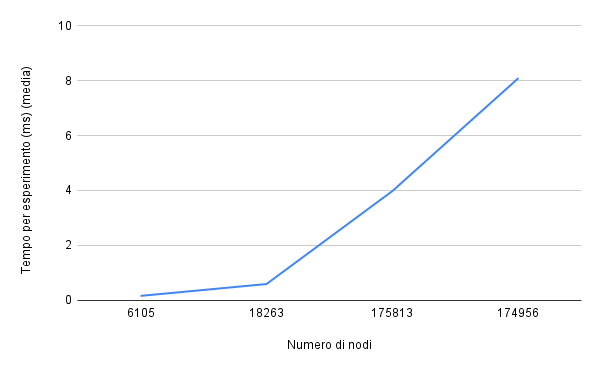
\includegraphics[width=1\textwidth]{Progetto Algoritmi/figures/tempo_nodi_gen.png}\captionof{figure}{\textbf{\small Tempo per esperimento, in millisecondi, rispetto al numero di nodi}}

\medskip

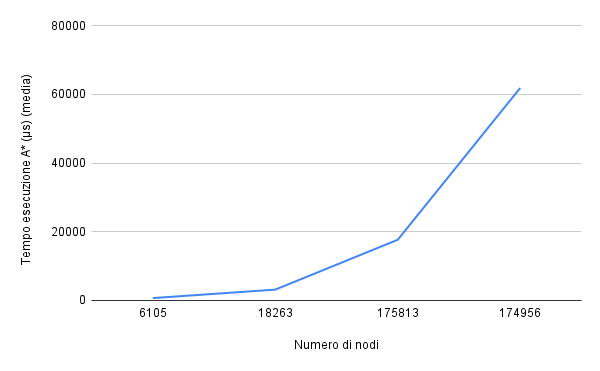
\includegraphics[width=1\textwidth]{Progetto Algoritmi/figures/tempo_nodi_astar.png}\label{img:tempo-nodi-astar}\captionof{figure}{\textbf{\small Tempo per una singola esecuzione di A*, in microsecondi, rispetto al numero di nodi}}

\medskip
\medskip
\medskip

Si può notare come i grafici nelle figure 4.1 e 4.2 descrivano un andamento simile per gli stessi valori dei nodi, ad evidenziare quindi che il comportamento asintotico del codice scritto, in questo caso, sia quello dell'algoritmo di pathfinding stesso. 

Per quanto riguarda la complessità si può vedere come il tempo di esecuzione si trovi tra una curva del tipo $y=nlog(n)$ ed un'altra del tipo $y=n$, ma servirebbero più dataset con numeri di vertici differenti per confermare.

Volendo vedere ora come cambiano i tempi di esecuzione relativamente all'utilizzo di un grafo orientato o non orientato, si vanno ad analizzare brevemente le figure di seguito.

\medskip

\includegraphics[width=1\textwidth]{Progetto Algoritmi/figures/tempo_probabilità_gen.png}\captionof{figure}{\textbf{\small Tempo per esperimento, in millisecondi, rispetto alla probabilità, aggregata tra dataset}}

\medskip
\medskip

\includegraphics[width=1\textwidth]{Progetto Algoritmi/figures/tempo_probabilità_astar.png}\captionof{figure}{\textbf{\small Tempo per una singola esecuzione di A*, in microsecondi, rispetto alla probabilità, aggregata tra dataset}}

Avendo ora sull'asse delle ascisse la probabilità, che in pratica rappresenta quanto il grafo sia vicino all'essere orientato o non orientato, si nota immediatamente come il doppio arco del grafo non orientato ($p=1$) migliori i tempi della ricerca del cammino minimo mostrati in figura 4.4. 
Guardando anche alla figura 4.3 si vede come il passaggio da $p=0.8$ a $p=1$ cambi l'ordine della curva, riducendone la complessità.

\medskip

\includegraphics[width=1\textwidth]{Progetto Algoritmi/figures/successi_probabilità.png}\captionof{figure}{\textbf{\small Percentuale di successi rispetto alla probabilità, aggregata tra dataset}}

\medskip

Infine si analizza il cambiamento della percentuale di successi, definiti come il riuscire a trovare un percorso tra due nodi presi casualmente, in relazione alla probabilità.
In questo caso si può notare il cambiamento sostanziale che ha passando da una $p=0.6$ a $p=0.8$ e ancora da $p=0.8$ a $p=1$.

%-----------------------------------------------%
% Sezione: Dataset reali di reti stradali [end] %
%-----------------------------------------------%

%--------------------------------------%
% Sezione: Grafi da modello ER [start] %
%--------------------------------------%
\section{Grafi da modello ER}\label{se:grafi-modello-ER}
In questa ultima sezione vengono invece analizzati i dati sperimentali relativi alla generazione dei grafi con il modello ER.
In questo caso la probabilità \textit{p} rappresenta la densità del grafo, con 0 per un grafo sparso ed 1 per archi tra tutte le coppie di nodi.

Dati i valori di \textit{p} ed \textit{n}, numero dei nodi nel grafo, per ogni set vengono eseguiti 1000 esperimenti che qui significano 1000 generazioni di grafi $G(n,p)$ diversi con conseguente scelta randomica dei nodi \textit{start} e \textit{goal}.
Il valore di \textit{n} varia da 25 a 500, con incrementi di 25, mentre \textit{p} va da 0 ad 1 con incrementi di 0.1.

Con questi valori di p si nota che non c'è interesse nell'analizzare la percentuale di successo di A* in quanto, come visto nella sezione sugli algoritmi di \hyperref[se:algo-gen-anal]{generazione di grafi}, per n abbastanza grandi la probabilità (densità) necessaria a far sì che il grafo sia connesso è molto piccola.

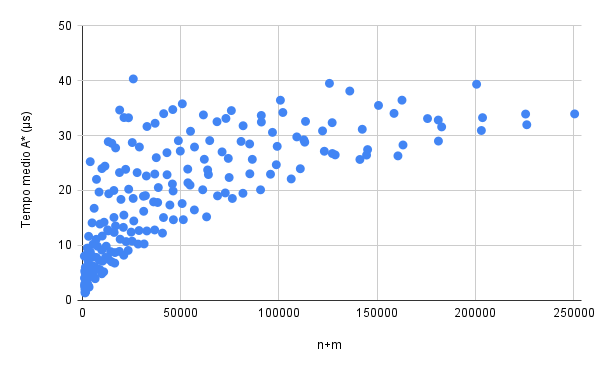
\includegraphics[width=1\textwidth]{Progetto Algoritmi/figures/tempo_vertici_archi.png}\captionof{figure}{\textbf{Tempo per una singola esecuzione di A*, in microsecondi, rispetto alla somma di nodi e archi}}

\medskip
\medskip

Volendo qui evidenziare il rapporto tra densità e tempo di esecuzione, nella figura 4.6 si fa un'analisi leggermente diversa rispetto alla \hyperref[img:tempo-nodi-astar]{precedente} e si vede come cambia il tempo necessario per una singola esecuzione di A* in base alla densità variabile. 
Si nota che la tendenza della curva, per n+m grandi, è simile a quella di $log(n)$.

\includegraphics[width=1\textwidth]{Progetto Algoritmi/figures/modulo_probabilità.png}\captionof{figure}{\textbf{Modulo della differenza tra distanza calcolata e distanza ottimale rispetto alla probabilità}}

\medskip
\medskip

In figura 4.7 invece viene evidenziato come al crescere della probabilità, e quindi della densità del grafo, il modulo della differenza tra distanza calcolata e distanza ottimale tenda scendere fino ad annullarsi. In applicazioni reali sarebbe quasi impossibile trovarsi nella situazione dove questo valore è uguale a zero in quanto significherebbe che esiste una strada che, presi qualsiasi due punti, li collega.
In questo caso il valore uguale a zero è dovuto allo spazio in cui vengono generate le coordinate X ed Y dei singoli nodi, ristretto 100000x100000 a tempo di esecuzione, che evidentemente causa un addensamento di vertici anche con un n massimo analizzato uguale a 500.

In realtà come visto nella relativa \hyperref[se:algo-path-anal]{sezione}, la condizione \textbf{\textit{$|f(x)-f^{*}(x)|=O(\log f^{*}(x))$}} è parte dei requisiti per avere una complessità polinomiale con A*. Di conseguenza si ipotizza che, potendo utilizzare uno spazio abbastanza ampio ed un livello di dettaglio maggiore per la probabilità ed essendo la l'euristica utilizzata efficace, il valore del modulo della differenza tra le distanze tenderà al logaritmo della distanza stimata.

%------------------------------------%
% Sezione: Grafi da modello ER [end] %
%------------------------------------%

%%%%%%%%%%%%%%%%%%%%%%%%%%%%%%%%%%%
%     Dati Sperimentali [end]     %
%%%%%%%%%%%%%%%%%%%%%%%%%%%%%%%%%%%

%%%%%%%%%%%%%%%%%%%%%%%%%%%%%%%%%%%%%%%%%%%%%
%     Bibliografia e Sitografia [start]     %
%                with BibTeX                %
%%%%%%%%%%%%%%%%%%%%%%%%%%%%%%%%%%%%%%%%%%%%%
\bibliographystyle{plain}
\bibliography{bibliografia}
%%%%%%%%%%%%%%%%%%%%%%%%%%%%%%%%%%%%%%%%%%%
%     Bibliografia e Sitografia [end]     %
%                with BibTeX              %
%%%%%%%%%%%%%%%%%%%%%%%%%%%%%%%%%%%%%%%%%%%


\end{document}
%%%%%%%%%%%%%%%%%%%%%%%%%%%%%%%%
%                              %
%     Begin Document [end]     %
%                              %
%%%%%%%%%%%%%%%%%%%%%%%%%%%%%%%%